\label{part2}
Lors de l'implémentation de notre projet, nous avons constaté qu'il nous faudrait passer les données dans deux réseaux différents pour obtenir une classification des types globules blancs à partir d'une image contenant des globules rouges, des globules blancs et du plasma, puisqu'il nous faut d'abord faire différencier globules blancs de globules rouges, puis faire apprendre les différents types de globules blancs à l'aide d'un jeu de données qui nous servirait de vérité terrain pour enfin obtenir notre classification de globules blancs.

\subsection{YOLO V5}
Nous avons utilisé YOLO V5 sans le jeu de données avec lequel il est présenté \footnote{\url{https://public.roboflow.com/object-detection/bccd}}, mais avons utilisé un guide d'utilisation \footnote{\url{https://colab.research.google.com/drive/1gDZ2xcTOgR39tGGs-EZ6i3RTs16wmzZQ}} pour l'adapter à notre jeu de données. L'algorithme présentant des résultats d'une précision et d'un taux de confiance d'environ 95\%, après une centaine d'epochs d'apprentissage nous n'avons pas tenté de pousser l'algorithme plus loin. Nous passons à l'algorithme des images de taille 416x416 et il nous sort un fichier texte pour chaque image avec le nom de l'image d'origine contenant une liste des plaquettes, des globules rouges et des globules blancs détectés, identifiés respectivement par 0, 1 ou 2, suivis des coordonnées du cadre dans lequel ils se trouvent.
\begin{figure}[!h]
    \centering
    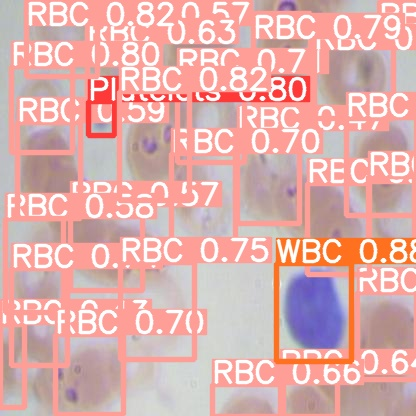
\includegraphics[scale=0.4]{images/yolo out.jpg}
    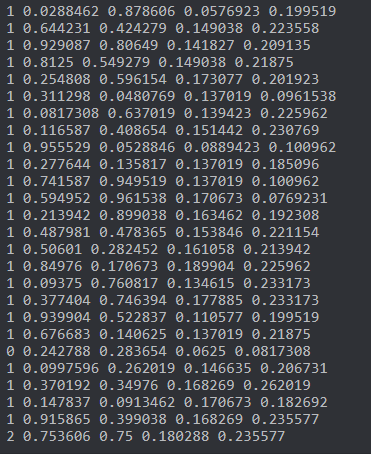
\includegraphics[scale=0.4]{images/yolo out txt.png}
    \caption{Output visuel et textuel de YOLO}
    \label{fig:yolo-out}
\end{figure}

\newpage
\subsection{Cutter}
Suite au passage dans l'algorithme YOLO V5, nous passons chaque image du jeu de données dans un algorithme de découpage. Cet algorithme prend en entrée les coordonnées de chaque globules blanc et l'extrait dans une nouvelle image. 
\begin{figure}[!h]
    \centering
    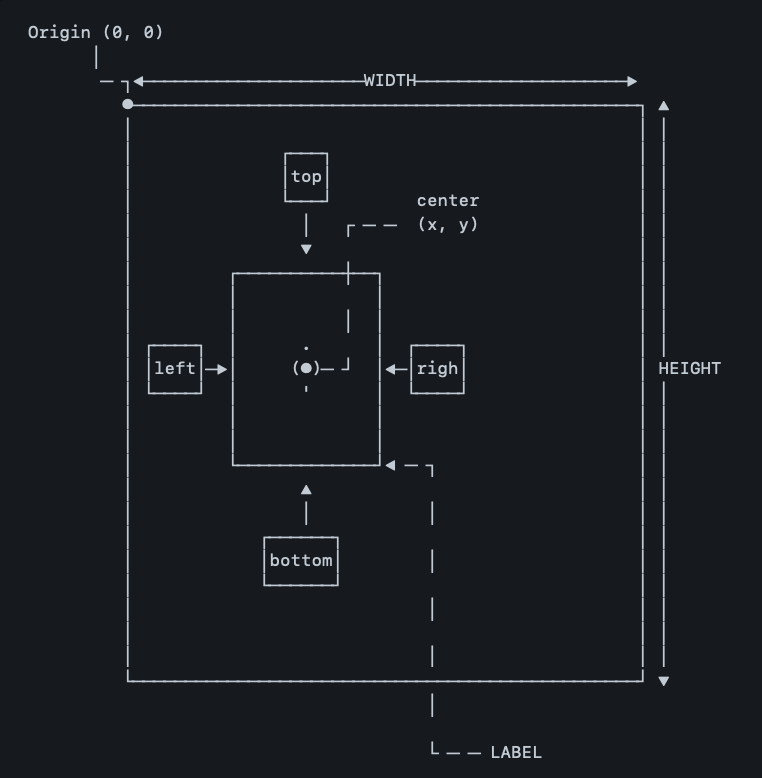
\includegraphics[scale=0.4]{images/cutter.png}
    \caption{Fonctionnement du cutter}
    \label{fig:cutter}
\end{figure}

\begin{figure}[!h]
    \centering
    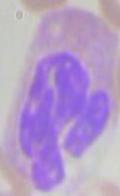
\includegraphics[scale=0.5]{images/postcut.jpeg}
    \caption{Image post cutter}
    \label{fig:postcutter}
\end{figure}

\subsection{Préprocessing avant classification}
Avant d'utiliser les images dans nôtres réseaux il est nécessaire de leur appliquer un pré traitement. Différentes approches ont été utilisées et nous allons, ici en discuter. Le problème des images utilisées en entrée du réseau, est qu’il y sont présents des globules rouges, en nombre plus ou moins important. Nous ne voulons pas que notre réseau prenne en compte ces cellules lors de la classification. Le but du pré traitement est d'isoler le noyau des cellules, qui est la partie qui permet de les différencier. Nous avons pris le temps d'inclure une explication plus détaillée du préprocessing dans le code source.
\paragraph{}
Une première approche à été de convertir l'image en niveau de gris puis de la binariser en prenant en compte un seuil. Cette approche permettait d’éliminer les globules rouges cependant il était possible d’utiliser d’autres outils afin de parvenir à un résultat plus correct. Pour ce faire, nous nous sommes intéressés aux mathématiques morphologiques. Ainsi, par le biais d’une alternance de dilatations et d’érosions nous sommes parvenus à un bien meilleur résultat qui aurait pu suffire, mais qui pouvait encore être amélioré.

\paragraph{}
Nous avons donc exploré la bibliothèque de scikit afin d’analyser les différentes options présentes. Il s’est avéré que scikit utilise une méthode bien plus efficace que la nôtre et nous en avons donc utilisé les fonctions pour finaliser notre algorithme. Une limite de l’algorithme est que certains noyaux ne sont pas parfaitement isolés et cela peut poser des problèmes.

\begin{figure}[!h]
    \centering
    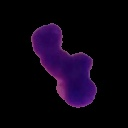
\includegraphics[scale=0.75]{images/globule cutter.jpg}
    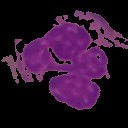
\includegraphics[scale=0.75]{images/globule cutter 2.jpg}
    \caption{Exemples de globules blancs préprocessés}
    \label{fig:wbc-preprocessed}
\end{figure}

\paragraph{}
Une fois cela fait, et pour indiquer au réseau quelles sont les classes de chaque image, nous avons fait le choix d’utiliser des DataGenerator. Le jeu de données choisi réparti chaque image de chaque type de cellule dans des dossiers distincts. Ainsi lors du chargement du fichier, et après avoir appliqué l’algorithme dessus, nous écrivons dans un fichier csv l’association du nom du fichier (son chemin plus exactement) associe à sa classe. La classe est un nombre compris entre 0 et 5.
\begin{itemize}
    \item 0 Basophile
    \item 1 Eosinophil
    \item 2 Lymphocyte
    \item 3 Monocyte
    \item 4 Neutrophil
\end{itemize}

\paragraph{}
Le réseau en lui-même est un CNN, nous avons étudié d’autres possibilités évoquées dans plusieurs articles tels que le W-NET mais le CNN utilisé étant suffisant nous n’avons pas choisi d’étudier la question plus en profondeur. Notre réseau, après une centaine d’epochs d’entraînement, affiche une 95\% d’efficacité.

\newpage